%\documentclass{article}
%\usepackage[a4paper, total={6in, 8in}]{geometry}
%\documentclass[reprint,amsmath,amssymb,rmp,onecolumn,notitlepage,11pt]{revtex4-1}
\documentclass[notitlepage,
reprint,%twocolumn,
%preprint
onecolumn,
amsmath,amssymb,superscriptaddress,aps,
pre,floatfix]{revtex4-1}
\usepackage[utf8]{inputenc}
%\usepackage{authblk}
%\usepackage{natbib}
\usepackage[normalem]{ulem}
\usepackage{graphicx}
\usepackage{hyperref}
\usepackage{xcolor}
\newcommand{\red}[1]{\textcolor{red!80!black}{#1}}
\newcommand{\blue}[1]{\textcolor{blue!80!black}{#1}}
\newcommand{\green}[1]{\textcolor{green!70!black}{#1}}
\newcommand{\gray}[1]{\textcolor{gray!80!black}{#1}}
\usepackage{mathtools}
\DeclarePairedDelimiter{\evdel}{\langle}{\rangle}
\usepackage[colorinlistoftodos]{todonotes}
\newcommand{\Pin}{P_{\mathrm{in}}}
\newcommand{\fhigh}{f_{\mathrm{high}}}
\newcommand{\flow}{f_{\mathrm{low}}}
\setlength {\marginparwidth }{2cm}


\begin{document}
\title{Supplementary material accompanying "Theory of chain separation distributions gives insights in real protein contact networks"}
\author{Nora Molkenthin}
\affiliation{Potsdam Institut für Klimafolgenforschung}
\affiliation{Center for Advancing Electronics Dresden (cfaed), Technical University of Dresden}
\author{J. J.  Güven}
\affiliation{EaStCHEM School of Chemistry, University of Edinburgh, Edinburgh, United Kingdom}
\author{Steffen Mühle}
\affiliation{Uni Göttingen, 37077 Göttingen, Germany}
\author{Antonia S J S Mey}
\email[Author to whom correspondence should be addressed: ]{antonia.mey@ed.ac.uk}
\affiliation{EaStCHEM School of Chemistry, University of Edinburgh, Edinburgh, United Kingdom}
\maketitle

\section*{Amino acid distance distributions of other chain lengths}
\subsection{AlphaFold 2}
Fig.~\ref{fig:alphafold} shows the amino acid distance distributions for protein contact maps calculated from AlphaFold 2~\cite{jumper2021highly} sequences in the chain length ranges of 85-115 (100), 185-215 (200) and 285-315 (300) amino acids. The plot shows the approximate power law behaviour of the distribution as well as the scaling with increasing chain lengths. 

\begin{figure*}[htb]
    \centering{
    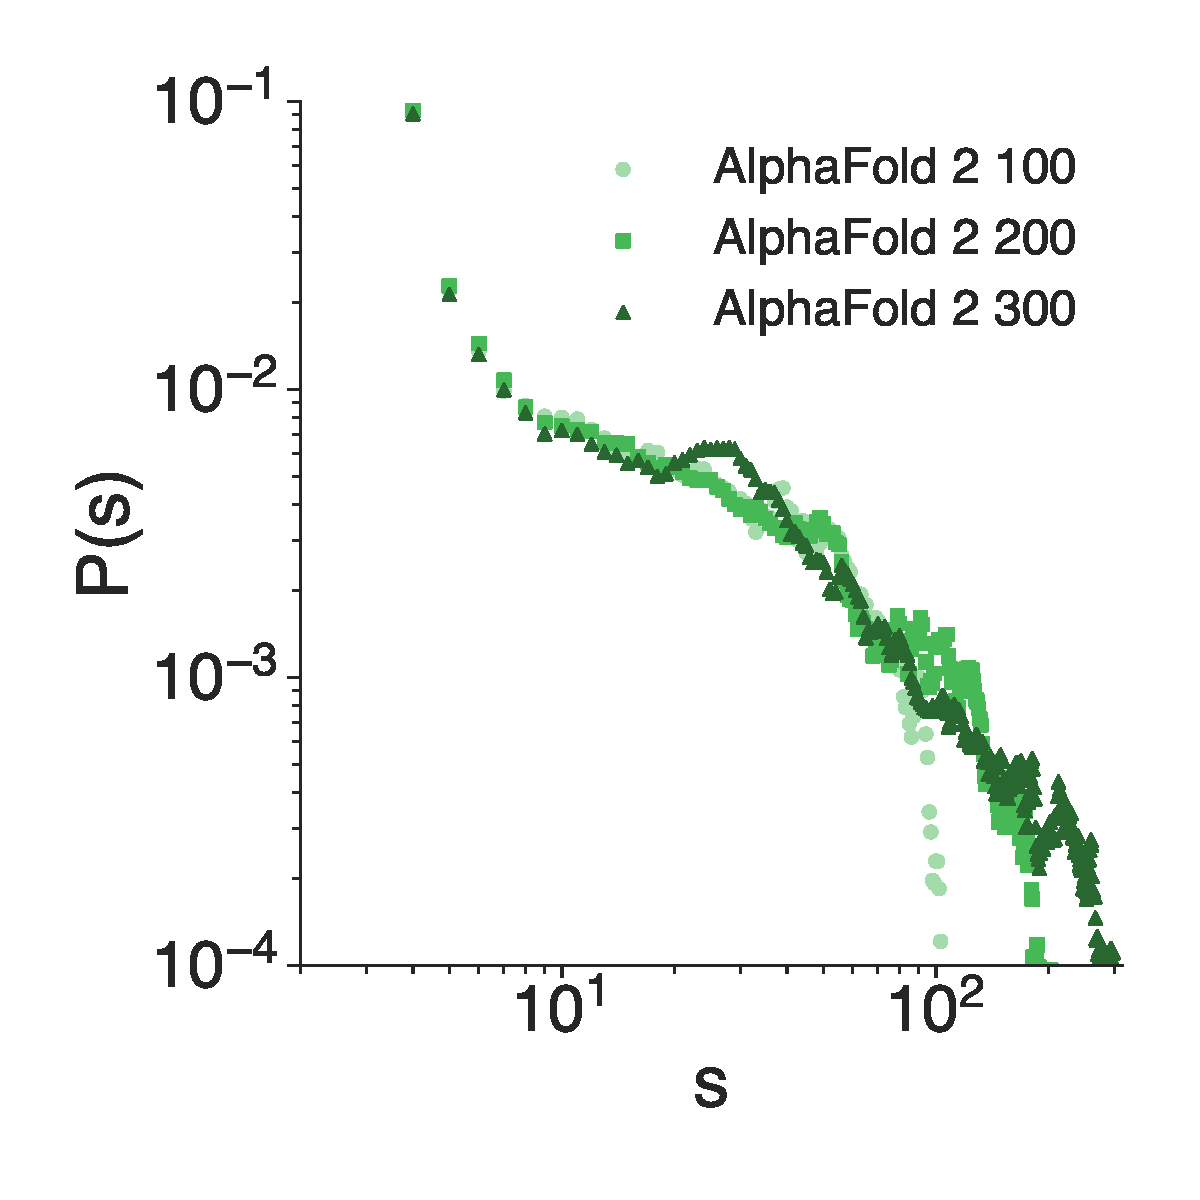
\includegraphics[scale=0.5]{paper/figures/SM_figures/alpha_chain_comparison.pdf}
    \caption{Amino acid distance distributions for contact maps derived from the AlphaFold 2~\cite{jumper2021highly} database for protein chains in the ranges of 85-115 (100), 185-215 (200) and 285-315 (300) amino acids.}
    \label{fig:alphafold}}
\end{figure*}

\subsection{Protein Data Bank and three-dimensional simulations}

Fig.~\ref{fig:rcsb_100} a shows the amino acid distance distributions for protein contact maps calculated from structures in the chain length range $\approx100$ for RCSB~\cite{PDB} (dark purple circles) and AlphaFold 2~\cite{jumper2021highly} (dark green squares). The shaded area shows the 95\% confidence level. Also shown are the analytic approximation and a general power law fitted to the RCSB data and their fit parameters, exponent $a$ and the dimensionality constant $A$ for the analytic approximation and exponent $\gamma$ for the power law,  are shown in~Table~\ref{table:stats} a. Similarly, Fig.~\ref{fig:rcsb_200} shows the amino acid distance distributions for protein contact maps calculated from structures in the chain length range $\approx200$ for RCSB~\cite{PDB}. We also computed the Kolmogorov-Smirnov (KS) statistic between the RCSB and AlphaFold 2 distributions for each length range. The KS statistics were 0.07 and 0.10 for the $\approx100$ and $\approx200$ ranges, respectively. For both of these, the null hypothesis was accepted at the $\alpha=0.01$ level.

Fig.~\ref{fig:sim_3d} shows the amino acid distance distributions for protein contact maps calculated from three-dimensional simulations obtained from~\cite{molkenthin2020self}. As before, the analytic approximation was fitted to the data in each range and the shaded area shows the 95\% confidence interval. The fit parameters $a$ and $A$ are given in Table~\ref{table:stats} c and d for ranges $\approx100$ and $\approx200$, respectively.

\begin{table}[tb]
\centering
\begin{tabular}{|c c c c c |}
\hline
Index & Data  & $A$ ($10^{-3}$) & $a$ & $\gamma$ \\
\hline
a & RCSB 100 & 1.5 $\pm$ 0.3  & 2 $\pm$ 1 &  0.83 $\pm$ 0.02\\
b & RCSB 200 & 0.8 $\pm$ 0.2 & 2 $\pm$ 1 & 0.95 $\pm$ 0.02 \\
c & 3D SIM 100 & 3.1 $\pm$ 0.6 & 2 $\pm$ 1 & --  \\
d & 3D SIM 200 & 1.2 $\pm$ 0.4 & 0.9 $\pm$ 0.9  & --  \\
\hline
\end{tabular}
 \caption{Parameters (exponent $a$ and dimensionality constant $A$) for the analytic approximation, exponent $\gamma$ for the power law fit, and their uncertainties from fitting to amino acid distributions obtained from RCSB proteins in the chain length range $\approx100$ a and $\approx200$ b amino acids. Shown also are the fit parameters $a$ and $A$ from fitting the analytic approximation to the 3D simulations~\cite{molkenthin2020self}. of chains in the $\approx100$ c and $\approx200$ d ranges.}
\label{table:stats}
\end{table}

\begin{figure*}[htb]
    \centering{
    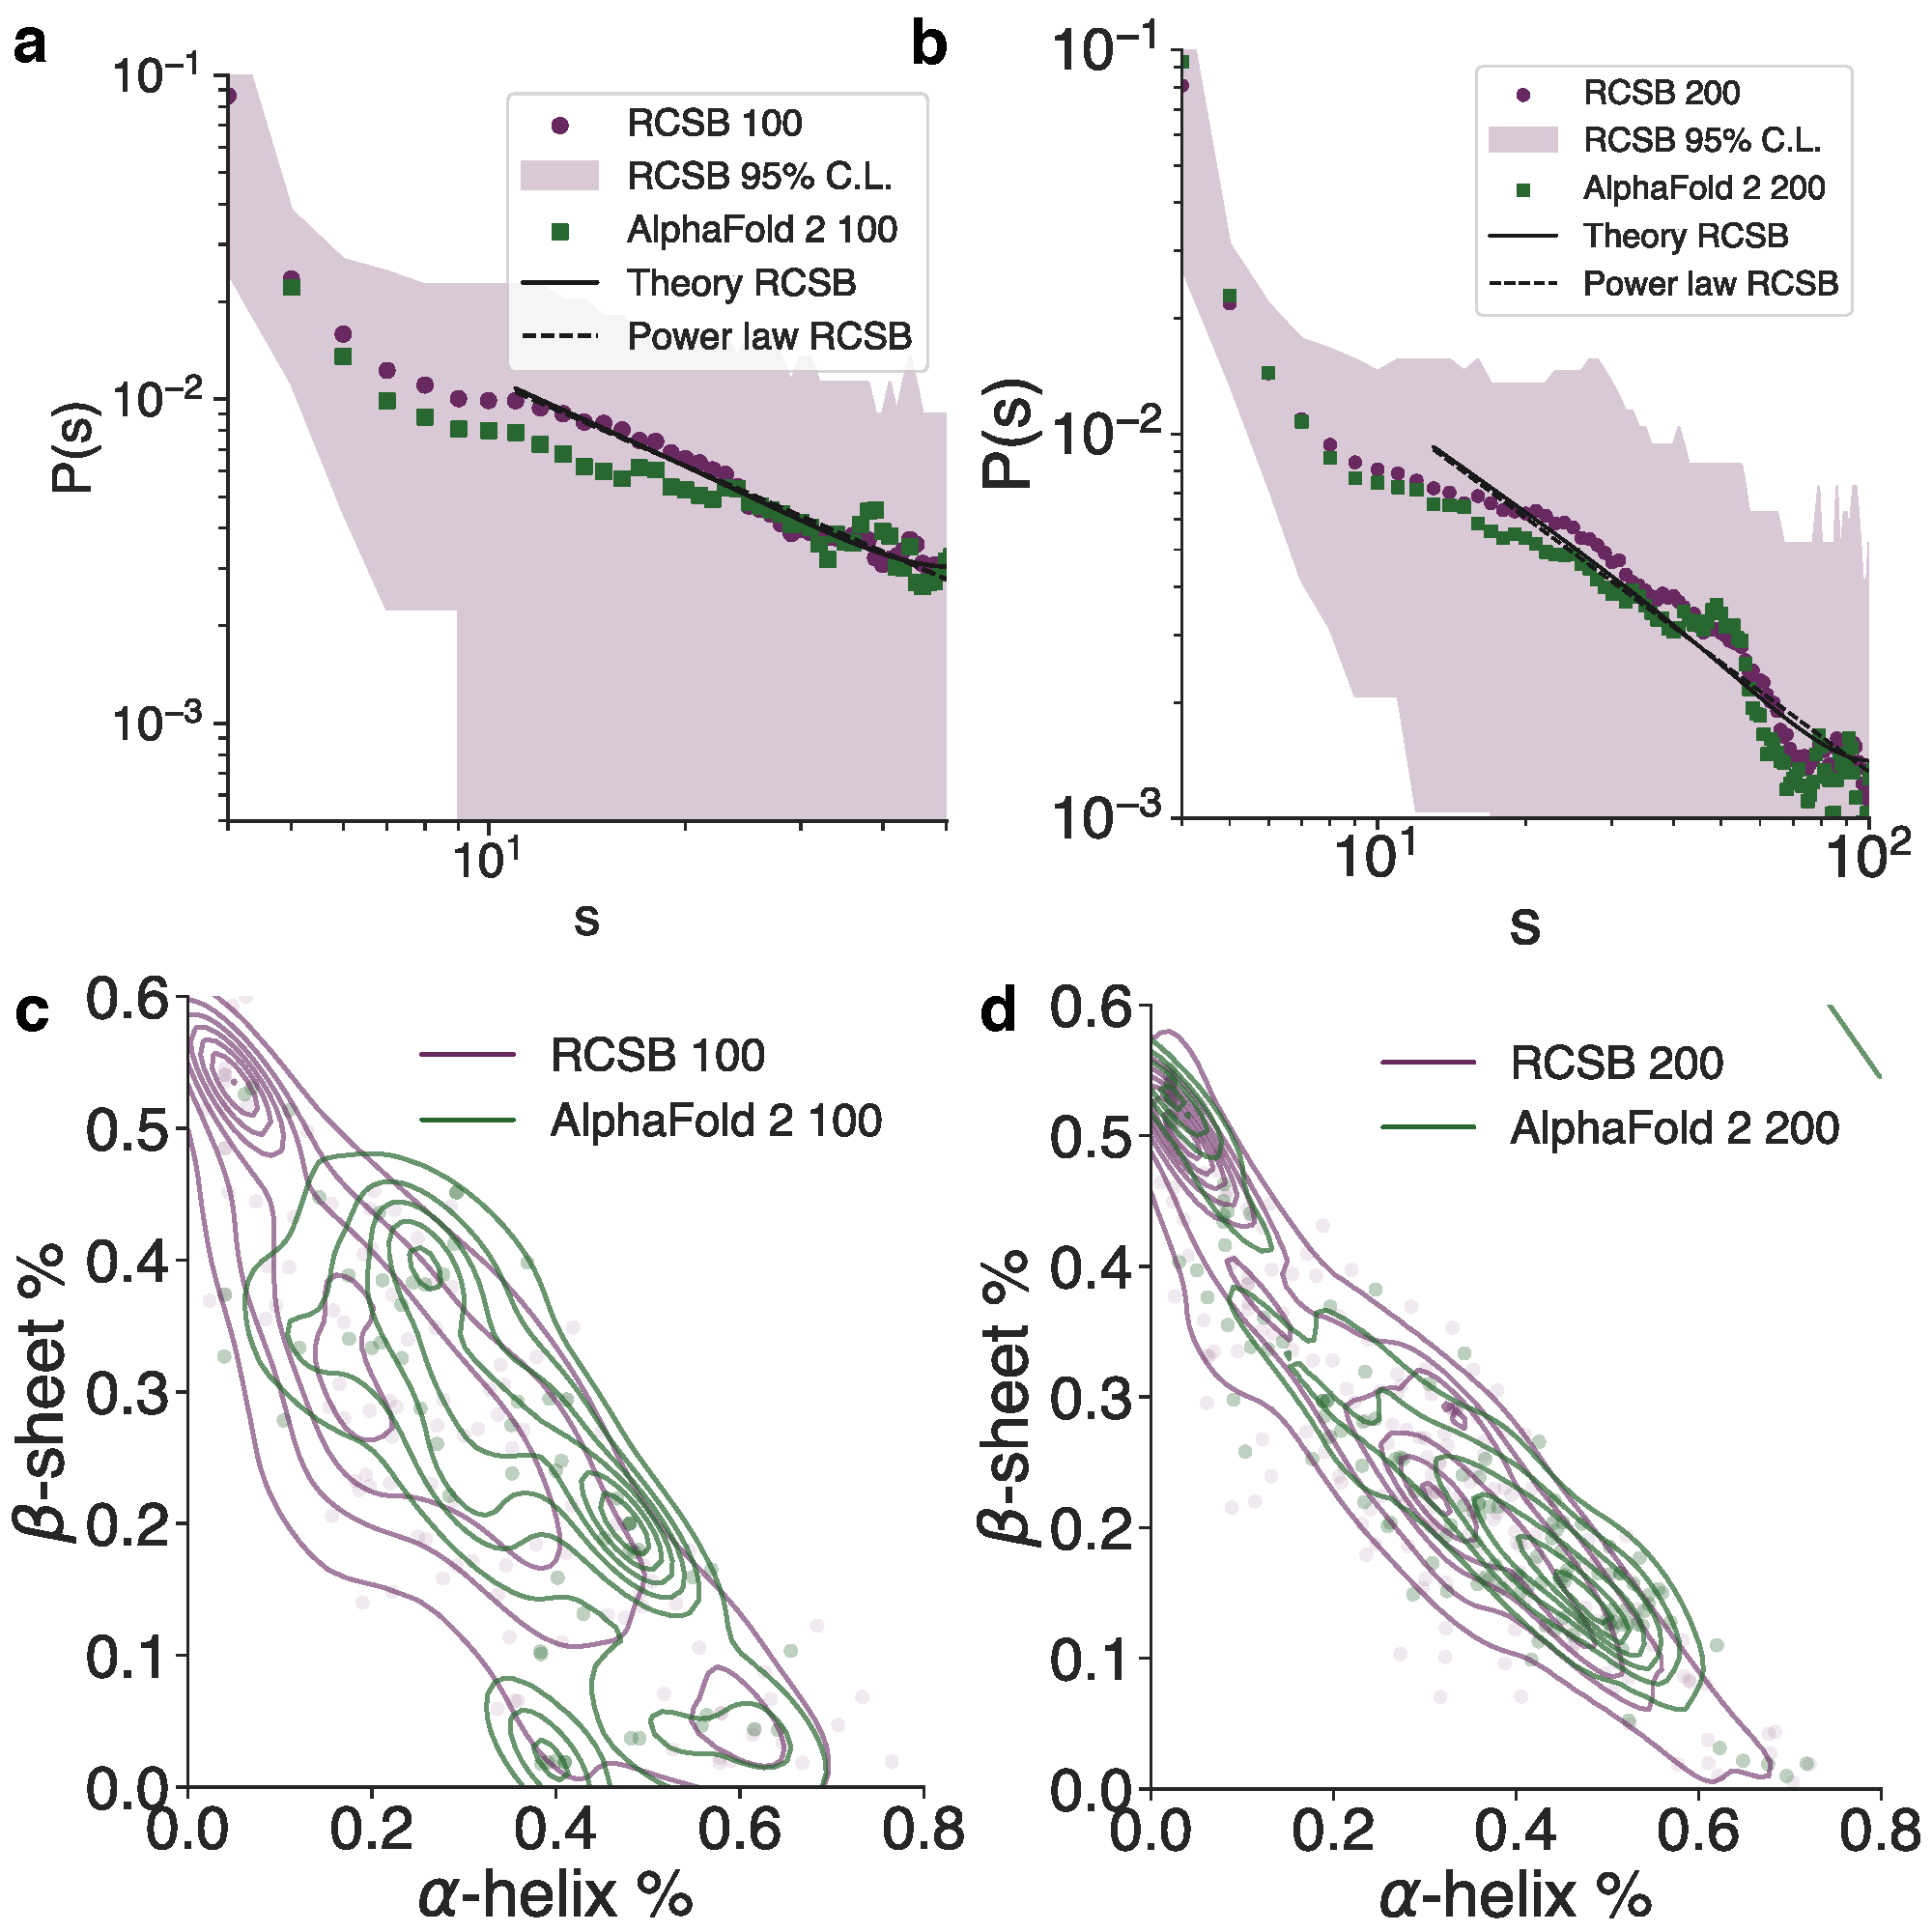
\includegraphics[scale=0.35]{paper/figures/SM_figures/distributions_combined.pdf}
    \caption{a) Comparison between the distributions of RCSB~\cite{PDB} and AlphaFold 2~\cite{jumper2021highly} databases for protein chains in the $\approx100$ range. The analytic approximation (solid line) and power law (dashed line) are fitted to the the RCSB data. Pink shaded area shows the 95\% confidence level. b) Secondary structure content distribution in the RCSB~\cite{PDB} and AlphaFold 2~\cite{jumper2021highly} structures in the $\approx100$ chain length range.}
    \label{fig:rcsb_100}}
\end{figure*}

% \begin{figure*}[htb]
%     \centering{
%     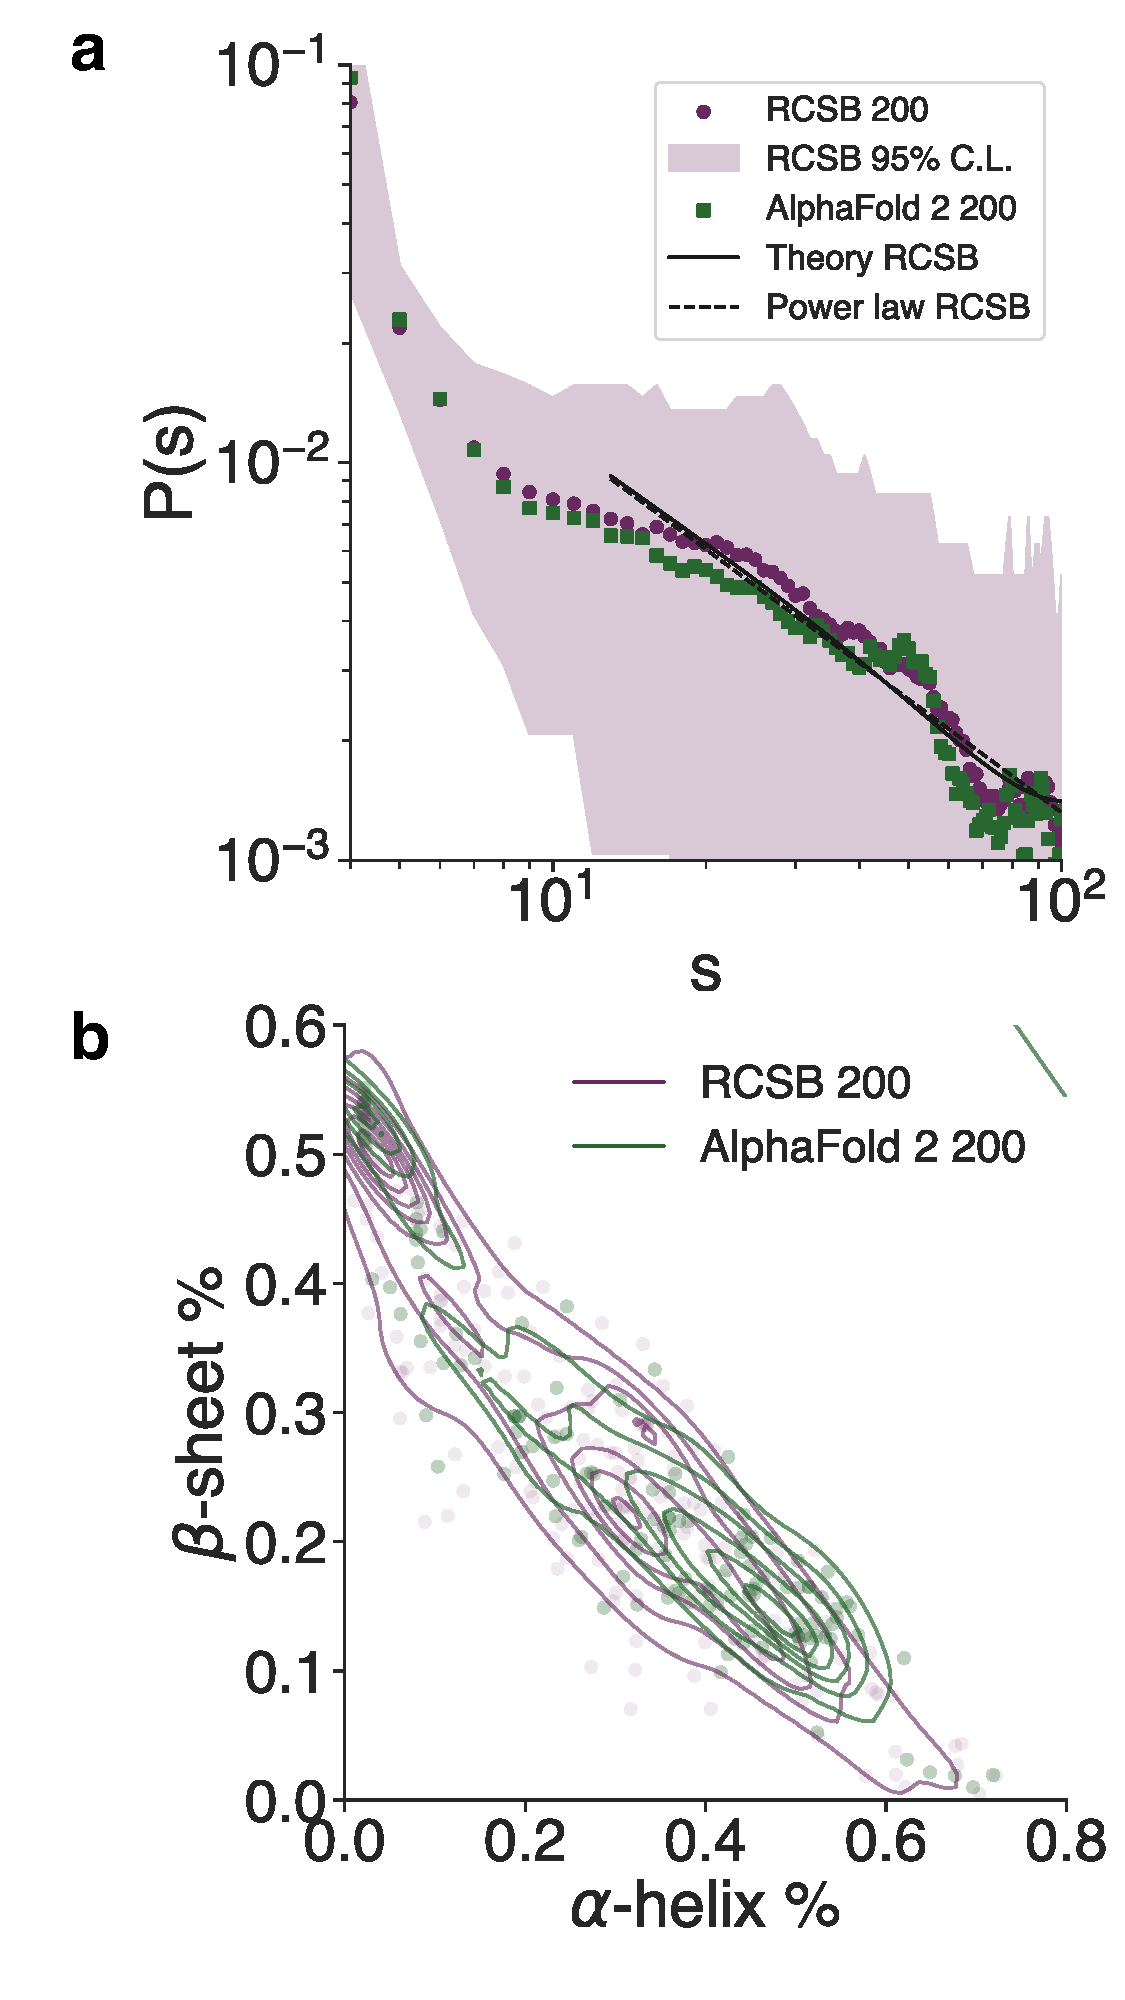
\includegraphics[scale=0.35]{paper/figures/SM_figures/distributions_200.pdf}
%     \caption{Comparison between the distributions of RCSB~\cite{PDB} and AlphaFold 2~\cite{jumper2021highly} databases for protein chains in the $\approx200$ range. The analytic approximation (solid line) and power law (dashed line) are fitted to the tail of the RCSB data. Pink shaded area shows the 95\% confidence level.}
%     \label{fig:rcsb_200}}
% \end{figure*}

\begin{figure*}[htb]
    \centering{
    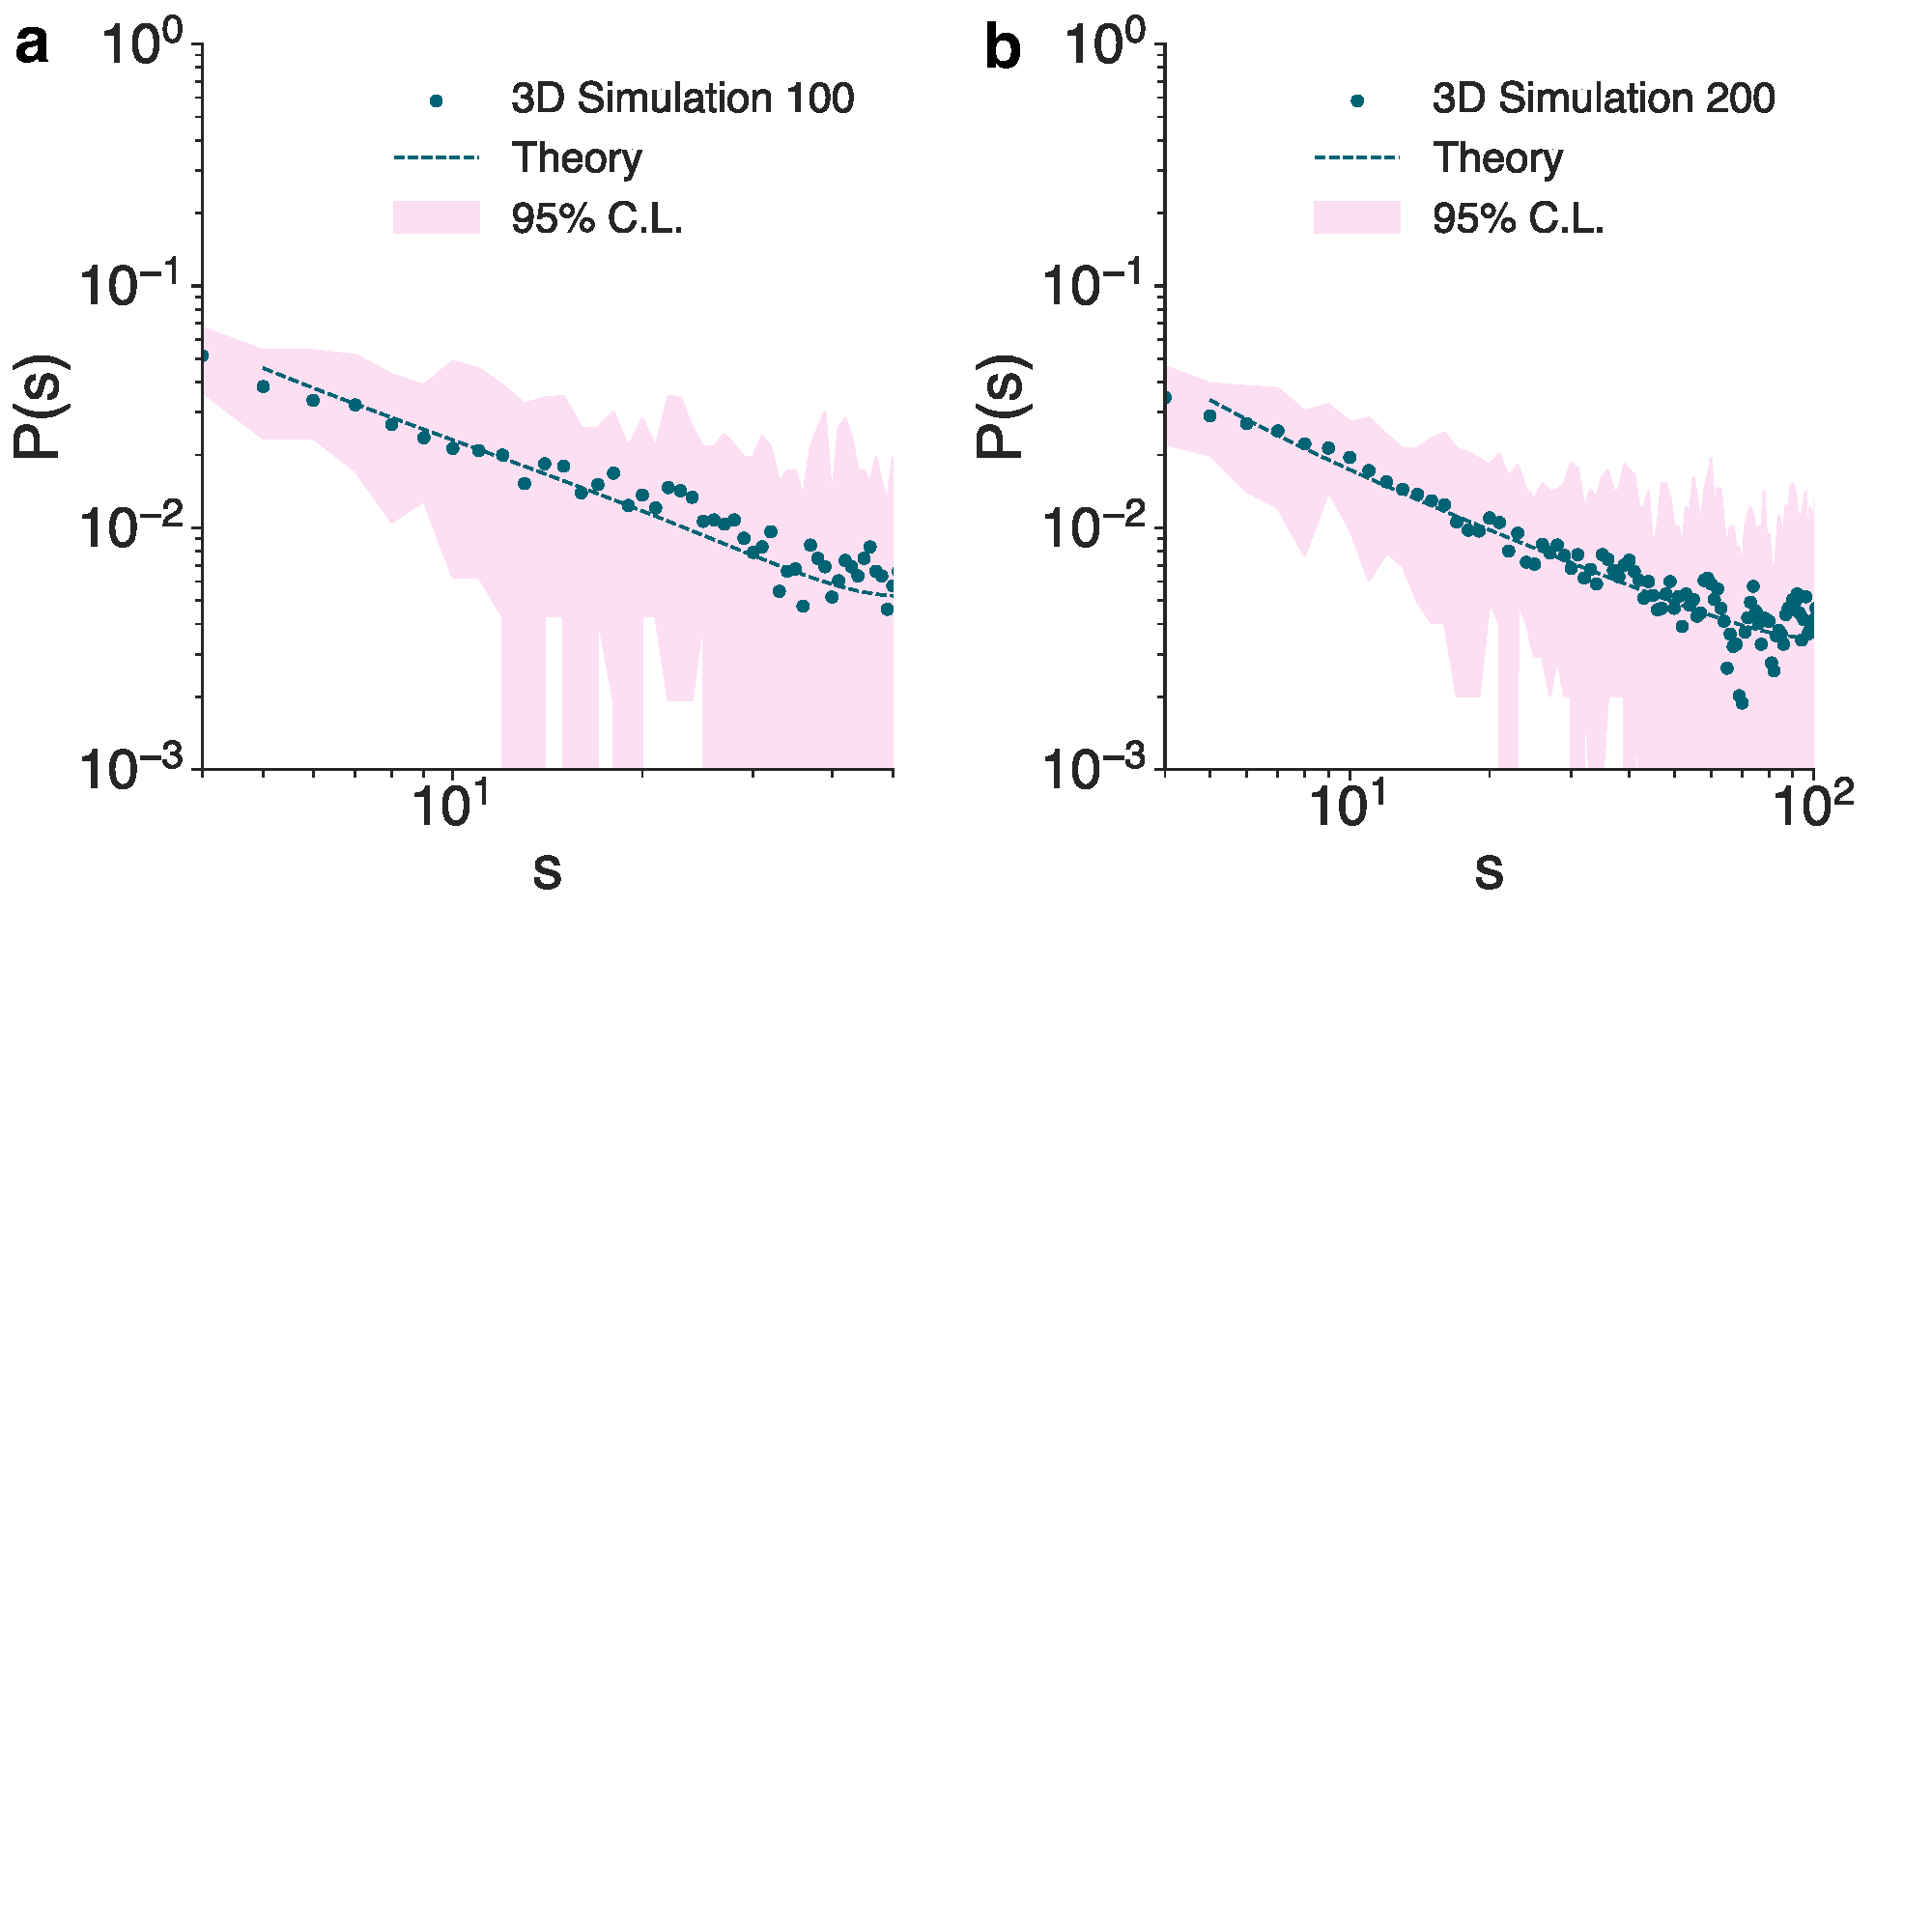
\includegraphics[scale=0.35]{paper/figures/SM_figures/simulations_3d.pdf}
    \caption{Amino acid distance distributions obtained from three-dimensional simulations~\cite{molkenthin2020self} for chains in the ranges $\approx100$ (a) and $\approx200$ (b) amino acids. The dotted line shows the analytic approximation fitted to the data and the shaded area shows the 95\% confidence level.}
    \label{fig:sim_3d}}
\end{figure*}



\newpage
\bibliographystyle{unsrt}
\bibliography{proteins}

\end{document}